\section{Combining FPGA and Processor}$~$ \\
Oftmals erfolgt die Kommunikation zwischen PS und PL über AXI. Die meisten IPs aus dem IP-Katalog von Xilinx haben diese Schnittstelle implementiert.

\subsection{SDK}$~$ \\
Mit dem SDK von Xilinx kann der ARM Prozessor auf dem Zynq programmiert werden. Wird das SDK gestartet, so öffnet sich automatisch ein neues generiertes Beispielprojekt.

\subsubsection{Benutzen der AXI Schnittstelle}
Im Beispielprojekt wird eine Datei \textit{xparameters.h} erstellt. Diese enthält Definitionen über die vorhandenen AXI-Schnittstellen, wie zum Beispiel der Adressbereich. In der Datei \textit{xil\_io.h} sind Funktionen enthalten um Register über AXI zu lesen und zu schreiben. Das SDK erstellt zudem in der Datei \textit{AXILite.h} oder \textit{AXI.h} spezialisierte Funktionen, welche passend auf die über AXI angeschlossenen Komponenten zugeschnitten sind (es wird deshalb empfohlen die Funktionen aus diesen Dateien zu benutzen).
\lstinputlisting[language=C,style=VHDL]{code/c/sdk_axi.c}

\subsubsection{AXI Direct Memory Access (DMA)}
Im IP Katalog von Xilinx gibt es einen AXI DMA IP Core. Dieser stellt zwei AXI4-Stream-Schnittstellen für eine hohe Bandbreite zur Verfügung. Eine Schnittstelle dient der Datenübertragung vom Master zum Slave, die andere für die gegengesetzte Richtung.

\begin{multicols}{2}
\paragraph{Verbindung mit ARM}$~$ \\
Um die beste  Performanz zu erreichen, sollte der IP Block wie nachfolgend dargestellt mit dem ARM verbunden werden:
\begin{figure}[H]
    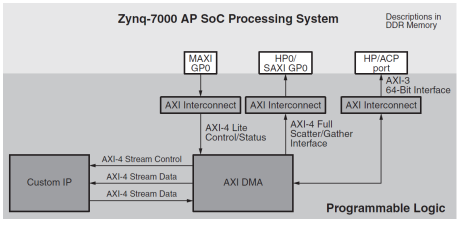
\includegraphics[width=0.5\textwidth]{images/sdk_dmaip.png}
\end{figure}

\paragraph{Modi}$~$ \\
Die folgenden Modi stellt der DMA IP Block zur Verfügung:
\begin{compactitem}
    \item \textbf{Register Direct Mode}: Dieser Modus wird benutzt, wenn eine hohe Geschwindigkeit zu einem Block im PL gefordert ist. Alle DMA Transfers werden gestartet, indem dem DMA-Blcok eine Ziel- oder Startadresse sowie eine Länge mitgeteilt wird. Sobald der Transfer abgeschlossen wurde, wird ein Interrupt generiert.
    \item \textbf{Scatter/Gatter Mode}: In diesem Mode werden Daten direkt in einen Speicher geschrieben, ohne dass vorher spezifisch eine Anforderung getätigt werden muss (benötigt mehr FPGA Ressourcen).
\end{compactitem}
\end{multicols}
\subsubsection{PL330 DMA}
Der Zynq stellt im PS einen eigenen DMA-Controller zur Verfügung. Bis zu acht Streams können von diesem Block gemanaged werden. Das SDK stellt in der Datei \textit{xdmaps.h} verschiedene Funktionen zur Ansteuerung des DMA-Controllers zur Verfügung.

\paragraph{DMA Schreibtransfer}
\lstinputlisting[language=C,style=C]{code/c/sdk_dmawrite.c}

\paragraph{DMA Lesetransfer}
\lstinputlisting[language=C,style=VHDL]{code/c/sdk_dmaread.c}
